\documentclass[journal,12pt,twocolumn]{IEEEtran}

\usepackage{setspace}
\usepackage{gensymb}
\singlespacing
\usepackage[cmex10]{amsmath}

\usepackage{amsthm}

\usepackage{mathrsfs}
\usepackage{txfonts}
\usepackage{stfloats}
\usepackage{bm}
\usepackage{cite}
\usepackage{cases}
\usepackage{subfig}

\usepackage{longtable}
\usepackage{multirow}

\usepackage{enumitem}
\usepackage{mathtools}
\usepackage{steinmetz}
\usepackage{tikz}
\usepackage{circuitikz}
\usepackage{verbatim}
\usepackage{tfrupee}
\usepackage[breaklinks=true]{hyperref}
\usepackage{graphicx}
\usepackage{tkz-euclide}

\usetikzlibrary{calc,math}
\usepackage{listings}
    \usepackage{color}                                            %%
    \usepackage{array}                                            %%
    \usepackage{longtable}                                        %%
    \usepackage{calc}                                             %%
    \usepackage{multirow}                                         %%
    \usepackage{hhline}                                           %%
    \usepackage{ifthen}                                           %%
    \usepackage{lscape}     
\usepackage{multicol}
\usepackage{chngcntr}

\DeclareMathOperator*{\Res}{Res}

\renewcommand\thesection{\arabic{section}}
\renewcommand\thesubsection{\thesection.\arabic{subsection}}
\renewcommand\thesubsubsection{\thesubsection.\arabic{subsubsection}}

\renewcommand\thesectiondis{\arabic{section}}
\renewcommand\thesubsectiondis{\thesectiondis.\arabic{subsection}}
\renewcommand\thesubsubsectiondis{\thesubsectiondis.\arabic{subsubsection}}


\hyphenation{op-tical net-works semi-conduc-tor}
\def\inputGnumericTable{}                                 %%

\lstset{
%language=C,
frame=single, 
breaklines=true,
columns=fullflexible
}
\begin{document}

\newtheorem{theorem}{Theorem}[section]
\newtheorem{problem}{Problem}
\newtheorem{proposition}{Proposition}[section]
\newtheorem{lemma}{Lemma}[section]
\newtheorem{corollary}[theorem]{Corollary}
\newtheorem{example}{Example}[section]
\newtheorem{definition}[problem]{Definition}

\newcommand{\BEQA}{\begin{eqnarray}}
\newcommand{\EEQA}{\end{eqnarray}}
\newcommand{\define}{\stackrel{\triangle}{=}}
\bibliographystyle{IEEEtran}
\raggedbottom
\setlength{\parindent}{0pt}
\providecommand{\mbf}{\mathbf}
\providecommand{\pr}[1]{\ensuremath{\Pr\left(#1\right)}}
\providecommand{\qfunc}[1]{\ensuremath{Q\left(#1\right)}}
\providecommand{\sbrak}[1]{\ensuremath{{}\left[#1\right]}}
\providecommand{\lsbrak}[1]{\ensuremath{{}\left[#1\right.}}
\providecommand{\rsbrak}[1]{\ensuremath{{}\left.#1\right]}}
\providecommand{\brak}[1]{\ensuremath{\left(#1\right)}}
\providecommand{\lbrak}[1]{\ensuremath{\left(#1\right.}}
\providecommand{\rbrak}[1]{\ensuremath{\left.#1\right)}}
\providecommand{\cbrak}[1]{\ensuremath{\left\{#1\right\}}}
\providecommand{\lcbrak}[1]{\ensuremath{\left\{#1\right.}}
\providecommand{\rcbrak}[1]{\ensuremath{\left.#1\right\}}}
\theoremstyle{remark}
\newtheorem{rem}{Remark}
\newcommand{\sgn}{\mathop{\mathrm{sgn}}}
%\providecommand{\abs}[1]{\left\vert#1\right\vert}
\providecommand{\res}[1]{\Res\displaylimits_{#1}} 
%\providecommand{\norm}[1]{\left\lVert#1\right\rVert}
%\providecommand{\norm}[1]{\lVert#1\rVert}
\providecommand{\mtx}[1]{\mathbf{#1}}
%\providecommand{\mean}[1]{E\left[ #1 \right]}
\providecommand{\fourier}{\overset{\mathcal{F}}{ \rightleftharpoons}}
%\providecommand{\hilbert}{\overset{\mathcal{H}}{ \rightleftharpoons}}
\providecommand{\system}{\overset{\mathcal{H}}{ \longleftrightarrow}}
	%\newcommand{\solution}[2]{\textbf{Solution:}{#1}}
\newcommand{\solution}{\noindent \textbf{Solution: }}
\newcommand{\cosec}{\,\text{cosec}\,}
\providecommand{\dec}[2]{\ensuremath{\overset{#1}{\underset{#2}{\gtrless}}}}
\newcommand{\myvec}[1]{\ensuremath{\begin{pmatrix}#1\end{pmatrix}}}
\newcommand{\mydet}[1]{\ensuremath{\begin{vmatrix}#1\end{vmatrix}}}
\numberwithin{equation}{subsection}
\makeatletter
\@addtoreset{figure}{problem}
\makeatother
\let\StandardTheFigure\thefigure
\let\vec\mathbf
\renewcommand{\thefigure}{\theproblem}
\def\putbox#1#2#3{\makebox[0in][l]{\makebox[#1][l]{}\raisebox{\baselineskip}[0in][0in]{\raisebox{#2}[0in][0in]{#3}}}}
     \def\rightbox#1{\makebox[0in][r]{#1}}
     \def\centbox#1{\makebox[0in]{#1}}
     \def\topbox#1{\raisebox{-\baselineskip}[0in][0in]{#1}}
     \def\midbox#1{\raisebox{-0.5\baselineskip}[0in][0in]{#1}}
\vspace{3cm}
\title{EE3025 Assignment-1}
\author{Koidala Surya Prakash - EE18BTECH11026}
\maketitle
\newpage
\bigskip
\renewcommand{\thefigure}{\theenumi}
\renewcommand{\thetable}{\theenumi}
Download all python codes from 
\begin{lstlisting}
https://github.com/Surya291/ACADEMIA/tree/master/IDP_3_2/Asst_01/codes

\end{lstlisting}
%
and latex-tikz codes from 
%
\begin{lstlisting}
https://github.com/Surya291/ACADEMIA/blob/master/IDP_3_2/Asst_01/Asst_01.tex
\end{lstlisting}


\section{Problem}
\begin{enumerate}[label=\thesection.\arabic*.,ref=\thesection.\theenumi]
    \numberwithin{equation}{enumi}
    
    \item Let
    \begin{align}
        x(n) = \cbrak{\underset{\uparrow}{1},2,3,4,2,1}
         \label{eq:equation0}\\
        y(n) + \frac{1}{2}y(n-1) = x(n) + x(n-2)	
        \label{eq:equation1}
    \end{align}
    
    \item Compute 
    \begin{align}
        X(k) \triangleq \sum_{n=0}^{N-1} x(n) e^{-j 2 \pi k n / N}, \quad k=0,1, \ldots, N-1
    \end{align}
    and $H(k)$ using h(n).
    
    \item Compute $X(k)$, $H(k)$ and $y(n)$ using FFT and IFFT methods.
\end{enumerate}
\section{Solution}
\begin{enumerate}[label=\thesection.\arabic*.,ref=\thesection.\theenumi]
\numberwithin{equation}{enumi}
\item
Computing h(n) using Z-transform of y(n) as follows : 
\begin{align}
    Y(z) + \frac{1}{2}z^{-1}Y(z)=X(z) + z^{-2}X(z)
\end{align}
\begin{align}
    \implies Y(z)=\frac{2(z^2+1)}{z(2z+1)}X(z)
\end{align}

\begin{align}
    H(z) = \frac{Y(z)}{X(z)} = \frac{1+z^{-2}}{1+\frac{1}{2}z^{-1}}
\end{align}

applying inverse Z-transform to compute $h(n)$
\begin{align}
 h(n)= Z^{-1}\left( {\frac{1}{1+\frac{1}{2}z^{-1}} + \frac{z^{-2}}{1+\frac{1}{2}z^{-1}}} \right)
\end{align}
\begin{align}
 h(n)={\frac{-1}{2}}^nu(n) + \left({\frac{-1}{2}}\right)^{n-2}u(n-2)
\end{align}

\item Computing y (for N samples) using FFT and IFFT : 

\begin{align}
X = FFT(x)\\
H = FFT(h)\\
Y = X.H\\
y = IFFT(Y)
\end{align}


\item If desired output is real : 
\begin{equation}
    y = IFFT(Y) = \frac{1}{N}*FFT(Y^{*})
\end{equation}

where $Y^{*}$ = complex conjugate(Y)\\
Thus IFFT can be implemented using the FFT function itself, which can save memory in a hardware setup.\\

\item Implementation and results : \\
y is computed through above steps (by padding x so that N = 8), while a recursive FFT algorithm is implemented to compute the 8 point FFT.\\
The code for it is as follows :
\begin{lstlisting}
https://github.com/Surya291/ACADEMIA/blob/master/IDP_3_2/Asst_01/codes/fft.py
\end{lstlisting}

\begin{equation}
\overline{x} =
\begin{bmatrix}
1\\2\\3\\4\\2\\1\\0\\0
\end{bmatrix} \hspace{10mm} 
\overline{h} =
\begin{bmatrix}
1. \\     -0.5 \\     1.25 \\   -0.625 \\   0.3125 \\ -0.15625 \\ 0.0625\\  -0.03125
\end{bmatrix}
\end{equation}


\begin{equation}
    \overline{X} =
\begin{bmatrix}
 13 \\   -3.121-6.536j \\  1.j \\     1.121-0.536j \\ -1.\\1.121+0.536j\\ -1.j\\    -3.121+6.536j
\end{bmatrix}
 \hspace{5mm}  \overline{H} =
\begin{bmatrix}
1.312+0.j \\    0.864-0.525j \\ 0.  \\    0.511+1.85j \\ 3.938 \\
 0.511-1.85j \\  0.  \\    0.864+0.525j
\end{bmatrix}
\end{equation}

\begin{figure}[!ht]

	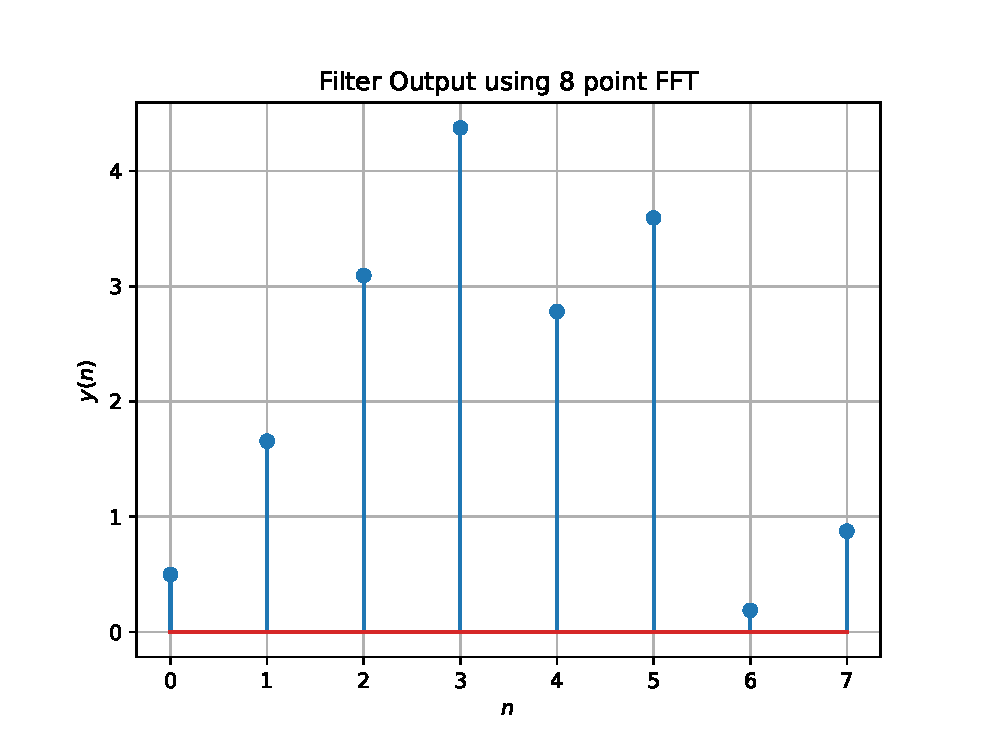
\includegraphics[width=10cm]{figs/fft.eps}
	\caption{y(n) obtained using 8 point recursive FFT}
\end{figure}
\bigskip

\item Formulating a recursive N-point FFT Algorithm \\ ( $N = 2^{\gamma};  \gamma$ is an integer ): 

    An N-point DFT can be written as : 
    \begin{align}
       X(k) &=  \sum_{n=0}^{N-1} x(n)e^{-j2\pi kn/N}, \quad k=0,1, \ldots, N-1 \\
    \end{align}
By dividing the inputs into even and odd indices ; where $W_{N} = e^{\frac{-j 2\pi }{N}} $

\begin{align}
\begin{split}
 X_{k} &=  \sum_{m=0}^{N/2 -1} x_{2m}e^{-\frac{j2\pi k2m}{N}} + \sum_{m=0}^{N/2 -1} x_{2m+1}e^{-\frac{j2\pi k(2m+1)}{N}}\\
       &=  \underbrace{\sum_{m=0}^{N/2 -1} x_{2m}e^{-\frac{j2\pi km}{N/2}}}_\text{ N/2 DFT with even inputs} + W_{N}^k \underbrace{\sum_{m=0}^{N/2 -1} x_{2m+1}e^{-\frac{j2\pi k(m)}{N/2}}}_\text{N/2 DFT with odd inputs}
\end{split}
\end{align}

While exploiting symmetry of $W_{N}$ as :

\begin{align}
  W_{N}^{k+N/2} = -W_{N}^k  
\end{align}

We can transform the iterative problem to a Divide-Conquer algorithm, where : 

\begin{align}
    X_{0\rightarrow \frac{N}{2}-1} = X_{even} + \overline{W}_{N/2}* X_{odd} \\
    X_{\frac{N}{2}\rightarrow N-1} = X_{even} - \overline{W}_{N/2} X_{odd} 
\end{align}

 $$\overline{W}_{N/2}(i) = W_{N}^i $$;  for i = 0,1,2 ... (N/2) -1 \bigskip\\
 
 Where $ X_{even}$ and $X_{odd}$ are again recursively computed using (N/2)-FFT thus halving its computation time;
until N = 2(the base case of the recursion) for which a 2-point DFT is computed as follows.

\begin{align}
    X = 
    \begin{bmatrix}
    1 & 1\\
    1& -1
    \end{bmatrix} * x
\end{align}

Thus , the time complexity of the algorithm is $O(Nlog_{2}N)$\bigskip

\item Vector representation of the FFT algorithm

An 8-point DFT can be represented as a Matrix product as follows:
$$\overline{X} = \overline{W}\;  \overline{x}$$

\begin{equation}
  \overline{x} =
\begin{bmatrix}
x(0) \\ x(1) \\ x(2) \\ x(3) \\ x(4) \\ x(5) \\x(6) \\x(7)
\end{bmatrix}  \hspace{5mm} \overline{X} =
\begin{bmatrix}
X(0) \\X(1) \\X(2) \\X(3) \\X(4) \\X(5) \\X(6) \\X(7) \\
\end{bmatrix} 
\end{equation}

\begin{equation}
\overline{W}
=
\begin{bmatrix}
W^{0} & W^{0} & W^{0} & W^{0} & W^{0} & W^{0} & W^{0} & W^{0} \\
W^{0} & W^{1} & W^{2} & W^{3} & W^{4} & W^{5} & W^{6} & W^{7} \\
W^{0} & W^{2} & W^{4} & W^{6} & W^{0} & W^{2} & W^{4} & W^{6} \\
W^{0} & W^{3} & W^{6} & W^{1} & W^{4} & W^{7} & W^{2} & W^{5} \\
W^{0} & W^{4} & W^{0} & W^{4} & W^{0} & W^{4} & W^{0} & W^{4} \\
W^{0} & W^{5} & W^{2} & W^{7} & W^{4} & W^{1} & W^{6} & W^{3} \\
W^{0} & W^{6} & W^{4} & W^{2} & W^{0} & W^{6} & W^{4} & W^{2} \\
W^{0} & W^{7} & W^{6} & W^{5} & W^{4} & W^{3} & W^{2} & W^{1} \\

\end{bmatrix}
\end{equation}

where $ W = W_{8} = e^{-j2\pi/8}$ \bigskip

The FFT algorithm exploits the inherent symmetry in $\overline{W}$ matrix by permuting $\overline{x}$ in a bit-reversed fashion.

A 8 point FFT can be represented as :

    $$\overline{X} = \overline{W_p}\;  \overline{x_p}$$\newline
    $$\overline{x}_{p} = P \; \overline{x}$$  
The P matrix rearranges the input x vector in a bit-reversed fashion as in : 
\begin{align}
    x_{p}(i) = x(\textit{bit reverse}(i)):
\end{align}
For Eg ; 
\begin{align}
\begin{split}
  x_{p}(4) = x_{p}(bin(100)) = x(bin(001)) = x(1)\\
\end{split}
\end{align}

\begin{equation}
    P = 
    \begin{bmatrix}
1 & 0 & 0 & 0 & 0 & 0 & 0 & 0 \\
0 & 0 & 0 & 0 & 1 & 0 & 0 & 0 \\
0 & 0 & 1 & 0 & 0 & 0 & 0 & 0 \\
0 & 0 & 0 & 0 & 0 & 0 & 1 & 0 \\
0 & 1 & 0 & 0 & 0 & 0 & 0 & 0 \\
0 & 0 & 0 & 0 & 0 & 1 & 0 & 0 \\
0 & 0 & 0 & 1 & 0 & 0 & 0 & 0 \\
0 & 0 & 0 & 0 & 0 & 0 & 0 & 1  

    \end{bmatrix}
\end{equation}

For such a rearrangement of $\overline{x}$ , we can exploit the symmetry in $W_{p}$, and thus factorise it into 3 sparse matrices.
\begin{equation}
    \overline{W}_{p} = \overline{W3} \; \overline{W2}\;\overline{W1}
\end{equation}


\begin{equation}
\overline{W3}
=
\begin{bmatrix}

1&.&.&.&W^{0}&.&.&. \\
.&1&.&.&.&W^{1}&.&. \\
.&.&1&.&.&.&W^{1}&. \\
.&.&.&1&.&.&.&W^{1} \\
1&.&.&.&-W^{0}&.&.&. \\
.&1&.&.&.&-W^{1}&.&. \\
.&.&1&.&.&.&-W^{1}&. \\
.&.&.&1&.&.&.&-W^{1} 

\end{bmatrix}
\end{equation}

\begin{equation}
\overline{W2}
=
\begin{bmatrix}
1&.&W^{0}&.&.&.&.&.\\
.&1&.&W^{2}&.&.&.&.\\
1&.&-W^{0}&.&.&.&.&.\\
.&1&.&-W^{2}&.&.&.&.\\
.&.&.&.&1&.&W^{0}&.\\
.&.&.&.&.&1&.&W^{2}\\
.&.&.&.&1&.&-W^{0}&.\\
.&.&.&.&.&1&.&-W^{2} 
\end{bmatrix}
\end{equation}

\begin{equation}
\overline{W1}
=
\begin{bmatrix}
1&W^{0}&.&.&.&.&.&. \\
1&-W^{0}&.&.&.&.&.&. \\
.&.&1&W^{0}&.&.&.&.\\
.&.&1&-W^{0}&.&.&.&.\\
.&.&.&.&1&W^{0}&.&.\\
.&.&.&.&1&-W^{0}&.&.\\
.&.&.&.&.&.&1&W^{0}\\
.&.&.&.&.&.&1&-W^{0}\\

\end{bmatrix}
\end{equation}

where (.) refers to zero.

Similarly a N-point DFT's W matrix can be factorised into $\gamma$ sparse matrices , ($N = 2^{\gamma}$) , with each row containing a 1 and a complex no. These $\gamma$ sparse matrices represent the $\gamma$-stages in the butterfly diagram of an N-point FFT.\\

\item Run time analysis of FFT  \bigskip

Considering no. of multiplications as a metric for time complexity:

1. In N-point DFT, the dense matrix multiplication consist of $2N^{2}$ real multiplications.
Hence time complexity of DFT is  \boldsymbol{$O(N^{2})$}\bigskip

2.While in FFT , there are logN(stages) sparse matrices, each stage requires 4*(N/2) real unique multiplications.\\
Thus, the total multiplications for N-FFT is 2*N*logN  which implies a time complexity of \boldsymbol{$O(NlogN)$}\bigskip

The below code compares time-complexities of DFT and FFT  :\begin{lstlisting}
https://github.com/Surya291/ACADEMIA/blob/master/IDP_3_2/Asst_01/codes/dft_vs_fft.py
\end{lstlisting}
 
 \begin{figure}[!ht]
	\includegraphics[width=10cm]{figs/dft_vs_fft.eps}
	\caption{Time complexity comparision}
\end{figure}

\item Convolution vs FFT\\
A convolution takes $ N^{2}$ operations $\approx \boldsymbol{O(N^{2})}$.\\
While the same output can be achieved using FFT and IFFT within : 
\begin{equation}
   \underbrace{O(NlogN)}_{\substack{\text{$x \rightarrow X$} \\ {\text{$h \rightarrow H $}}  }} + 
   \underbrace{O(N)}_{\text{$Y = X*H$}} + 
   \underbrace{O(NlogN)}_{\text{$Y \rightarrow y$}} \approx \boldsymbol{O(NlogN)}
\end{equation}

\end{enumerate}
\end{document}
